
\subsection{Application on MNIST}
In this section we show result for applying unsupervised Convolutional Sparse Coding (denoted as CSC) presented before on MNIST dataset.
\begin{figure}[h]
 \centering
 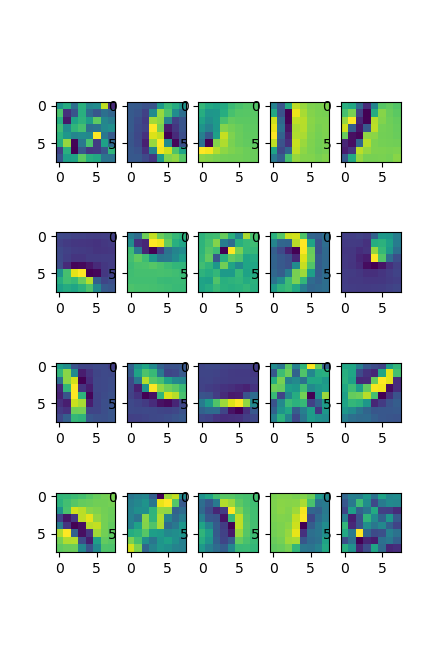
\includegraphics[scale=0.6]{../Results/SPORCO_MNIST/D.png}
 % D.png: 445x648 px, 100dpi, 11.30x16.46 cm, bb=0 0 320 467
 \caption{Filters from D}
\end{figure}
\begin{figure}[h]
 \centering
 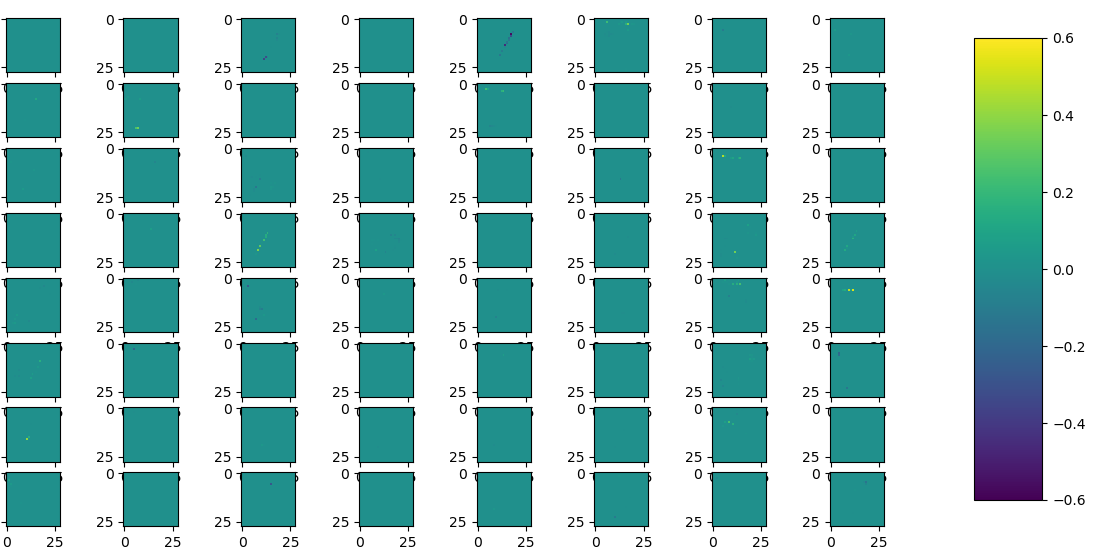
\includegraphics[scale=0.6]{../Results/SPORCO_MNIST/activation.png}
 % CartesActivations.png: 663x648 px, 100dpi, 16.84x16.46 cm, bb=0 0 477 467
 \caption{Activation map}
\end{figure}



 \begin{figure}[h]
 \begin{subfigure}{.5\textwidth}
 \centering
 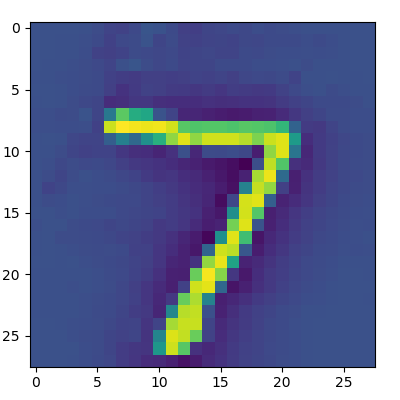
\includegraphics[scale=0.5]{../Results/SPORCO_MNIST/reconstruction.png}
  %\caption{Reconstructed 7 vs Original 1}
 % module-capteur-laser.jpg: 600x600 px, 72dpi, 21.17x21.17 cm, bb=0 0 600 600
 \end{subfigure}%
  \begin{subfigure}{.3\textwidth}
 \centering
 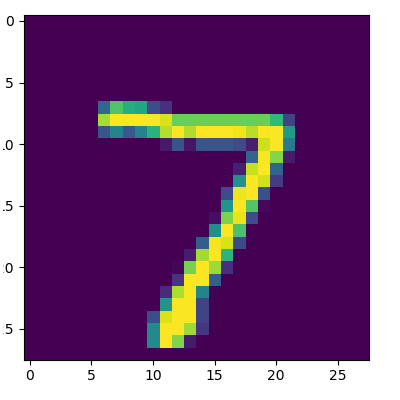
\includegraphics[scale=0.5]{../Results/SPORCO_MNIST/Original.png}
 % module-capteur-laser.jpg: 600x600 px, 72dpi, 21.17x21.17 cm, bb=0 0 600 600
  %\caption{Reconstructed 3 vs Original 3}

 \end{subfigure}%

\caption{Reconstructed 7 vs Original 7}
 \end{figure}


\newpage
\subsection{Discussion}
Using this examples we validate that CSC allow us to reconstruct our input data using filters, convolutions and activation maps. But we still cannot use activation maps for clustering or classification due to the non-discriminative reconstruction. Indeed, two seven in our test dataset haven't the same decomposition ( i.e. they don't have the same or close activation maps).
